\documentclass[11pt,a4paper]{article}

\usepackage[utf8]{inputenc}
\usepackage{amsmath,amssymb,amsthm}
\usepackage{mathtools}
\usepackage[margin=1.1in]{geometry}
\usepackage{graphicx}
\usepackage{booktabs}
\usepackage{array}
\usepackage[hyphens]{url}
\usepackage{hyperref}

\theoremstyle{plain}
\newtheorem{lemma}{Lemma}

\newcommand{\FF}{\mathbb{F}}
\newcommand{\GL}{\mathrm{GL}}
\newcommand{\Sdir}{\texttt{S/}}
\newcommand{\Lhat}{\hat{L}}
\urlstyle{tt}
\emergencystretch=2em

\title{Small-prime splitting of the NIST/ANSI prime-field curves:\\
a prime-order null, a cutoff sweep, and a held-out test}
\author{Anonymous}
\date{30 October 2026}

\begin{document}
\maketitle

\begin{abstract}
A retrospective observation holds that the published 1997--98 NIST/ANSI
prime-field curves have fewer \emph{split} small primes than the eleven named
prime-order seed candidates passed over in the same generator streams. A split
prime is an odd prime $\ell \le 691$ at which $\Delta = t^2 - 4p$ is a nonzero
square. The most extreme case is prime239v1, with 42 splits against 61--71 for
the five omitted 239-bit curves. We test three objections.
(i)~\emph{Prime-order confound.} All nineteen curves have prime order, so no
omitted curve gains forced splits from small factors of $n$. Under an exact
Chebotarev null conditioned on prime order, the mean split count is
59.7--60.2 (s.d.\ 5.5), not 62. The prime-order correction is 0.5--1.4
splits, and small factors of the twist order contribute 0--4 forced splits per
curve. Neither explains the gap.
(ii)~\emph{Cutoff choice.} On the nineteen curves, a within-field pair score of
25/25 occurs only for $B \in \{691, 701, 709, 769\}$; elsewhere it is 19--23.
A look-elsewhere correction over 655 prime cutoffs still leaves
$p \approx 0.006$.
(iii)~\emph{Replication.} We fixed the statistic at $B = 691$ in a protocol
committed before the data, then applied it to the 42 unpublished
draft-eligible curves in the same streams that were \emph{not} among the named
eleven. The association \textbf{does not replicate}: held-out curves exceed
published ones in 0.574 of 102 within-field pairs (one-sided permutation
$p = 0.29$).
What survives is a single low outlier, prime239v1, at the 0.06th percentile.
Among the 61 eligible curves examined, a minimum that extreme has null
probability about 0.05. Its $L(1,\chi_{D_K})$ is also low, but this is the
same anomaly in another weighting, and its class number is far from the scale
a CM-method generator produces. No known mechanism links rational small
isogenies to discrete-logarithm hardness. We find no evidence of a split-count
selection rule.
\end{abstract}

\paragraph{Evidence.} Every number below cites a committed artefact in
\path{crypto-autoresearcher:research/nist_seed_split_null_20261029/}
(abbreviated \Sdir{} here) or in one of the studies named in Section~\ref{sec:data}.

\section{The claim under test}

The recovered \texttt{lrand48}/SHA-1 seed streams behind the X9.62/NIST
prime-field curves~\cite{x962draft1997} contain prime-order candidates that
were never published. Eleven of them have been named as \emph{omitted}: five
239-bit, three P-224, two 192-bit and one P-256. They have been compared with
the eight published curves of the same fields (prime192v1--v3, secp224r1,
prime239v1--v3, prime256v1).
\path{crypto-autoresearcher:problems/nist-seed-selection-rule-unexplained.md}
lists the many features already tested on these nineteen curves.

For a curve with trace $t = p + 1 - n$, the observation counts
\begin{equation}
  S(E) = \#\{\, \ell \text{ odd prime},\ 3 \le \ell \le 691 : (\Delta/\ell) = +1 \,\},
  \qquad \Delta = t^2 - 4p .
\end{equation}
A split prime is an Elkies prime~\cite{schoof1995}: Frobenius has eigenvalues
in $\FF_\ell$, and $E$ has two rational $\ell$-isogenies. The reported pattern
is that published curves have smaller $S$ in every same-field comparison. A
critique raised three problems: a prime-order confound, forking paths (the
cutoff 691, the ramified convention, a sign test over four fields), and the
lack of a mechanism.

\paragraph{Related work.} The seeds were traced to a timestamp-seeded
\texttt{lrand48} generator, and the omitted candidates were identified, by an
Anthropic Frontier Red Team study~\cite{anthropic2026seeds} and by
Valsorda~\cite{valsorda2026seeds}. Valsorda reports one undocumented
rejection rule, that a candidate whose order has more bits than the field is
skipped. He finds no rule for the remaining surplus, and estimates the
selector had about 30 bits of freedom. Neither study tests an arithmetic
property such as split or Elkies primes, the CM discriminant or the class
number, on published against omitted curves. Bernstein et al.~\cite{bada55}
showed how seed search lets a standard select curves with rare properties;
SafeCurves~\cite{safecurves} requires a CM discriminant
$|D| > 2^{100}$, which every curve here meets. On average over curves, Elkies
and Atkin primes occur in equal proportion~\cite{shparlinski-sutherland}. We
found no earlier test of split counts, or of $L(1,\chi_{D_K})$, on these
curves.

\section{Data}\label{sec:data}

\begin{itemize}
\item \textbf{Nineteen named curves.} Exact $p$, $n$ and EC1 curve UIDs come
  from \path{research/nist_seed_1997_selection_extension_20261023/sea_signature/runs/scan-20261023T1840Z/raw.json}
  (SHA-256 \texttt{4a0df1de\ldots48fe}). That study independently verified the
  Legendre symbols in Sage. Every $n$ is prime.
\item \textbf{Held-out cohort.}
  \path{research/nist_seed_1997_acceptance_20261024/analysis.json} classifies
  69 seed positions whose curves pass the November 1997 X9.62 draft's
  numerical checks with certified prime order. Of these, 10 are published and
  59 unpublished; the named eleven are a retrospective subset of the 59. The
  other 48 unpublished positions (\texttt{order\_too\_wide\_only},
  \texttt{opposite\_root\_only}) never entered the 691 observation. Of those,
  42 lie in the four comparison fields and 6 in P-384. Fifteen of the 42
  (\texttt{order\_too\_wide\_only}) fall under Valsorda's bit-length
  rule~\cite{valsorda2026seeds}, so they have a documented, innocuous reason
  for being passed over.
\item \textbf{Held-out $p$ and $n$} come from the certified branches in
  \path{research/nist_seed_selection_20261016/raw/full_prime_order_certificates.jsonl}.
  The two square-root branches at one seed are isomorphic or quadratic twists
  ($t \mapsto \pm t$), so they share $\Delta$ (asserted in
  \path{S/heldout.py}).
\end{itemize}

\section{A prime-order null}\label{sec:null}

\begin{lemma}
Let $\ell$ be an odd prime with $\ell \mid n = p + 1 - t$. Then
$t \equiv p + 1$ and $\Delta \equiv (p-1)^2 \pmod{\ell}$, so $\ell$ splits
unless $p \equiv 1 \pmod{\ell}$, in which case it ramifies. The same holds
when $\ell$ divides the twist order $p + 1 + t$.
\end{lemma}

Both groups have prime $n$, so the lemma cannot separate them through $n$. The
twist orders do have small odd factors $\le 691$ on 18 of 19 curves (0--4 per
curve). The published curves have no fewer of these, averaging 2.0 against
1.7. Excluding those primes leaves the results unchanged
(\path{S/runs/results.json}, variant \texttt{split-twist}).

\paragraph{Null.} For a random curve over $\FF_p$ and a small $\ell \ne p$,
Frobenius mod $\ell$ is asymptotically distributed like a uniform matrix in
$\GL_2(\FF_\ell)$ with determinant $p$~\cite{castryck-hubrechts}. The number of
$2\times 2$ matrices over $\FF_\ell$ with trace $u$ and determinant $d$ is
$\ell^2 + \ell\,\chi(u^2 - 4d)$. Prime order excludes the eigenvalue~1, that
is $u \equiv 1 + d$. Hence
\begin{equation}
  P_\ell(\text{split}) =
  \frac{\sum_{u \not\equiv 1+d,\ \chi(u^2-4d)=1} (\ell^2 + \ell)}
       {\sum_{u \not\equiv 1+d} \bigl(\ell^2 + \ell\,\chi(u^2-4d)\bigr)} .
\end{equation}
Assuming independence across $\ell$ gives an exact Poisson-binomial law for
$S$ in each field. A curve's position is its mid-percentile
$100\cdot\bigl(P(X < S) + P(X = S)/2\bigr)$.

\begin{table}[ht]
\centering
\begin{tabular}{lrrrr}
\toprule
Field & Mean, all curves & Mean, prime order & Shift & s.d., prime order \\
\midrule
192-bit & 61.08 & 59.70 & $-1.38$ & 5.51 \\
224-bit & 60.62 & 60.08 & $-0.53$ & 5.53 \\
239-bit & 61.12 & 59.72 & $-1.40$ & 5.51 \\
256-bit & 60.69 & 60.18 & $-0.51$ & 5.54 \\
\bottomrule
\end{tabular}
\caption{Null split count over the 124 odd primes $3 \le \ell \le 691$.
Source: \texttt{S/runs/results.json}.}
\label{tab:null}
\end{table}

\paragraph{Validation.}
\begin{itemize}
\item \emph{48-bit sample.} PARI SEA counts of 1{,}500 prime-order curves
  $y^2 = x^3 - 3x + b$ over each of two random 48-bit primes matched the model:
  means 60.11 and 60.08 against 60.20 and 60.30, KS distances 0.023 against a
  5\% critical value of 0.035 (\path{S/runs/validation48_stdout.log}). The
  first run kept only aggregates (deviation D2 in \path{S/DEVIATIONS.md}). A
  rerun with the same seed reproduced both output lines exactly and saved all
  3{,}000 rows (\path{S/runs/validation48_rows.jsonl.gz}). An independent
  audit recomputed every statistic from the rows and re-counted 100 curves
  with PARI, with 0 mismatches (\path{S/runs/validation48_audit.json}).
\item \emph{Real fields.} The 42 held-out curves give a second check, over the
  real fields (Section~\ref{sec:heldout}).
\item \emph{Not done.} A 10{,}000-curve SEA sample per real field remains open.
\end{itemize}

\section{Exploratory analysis of the nineteen curves}\label{sec:explore}

\begin{figure}[ht]
\centering
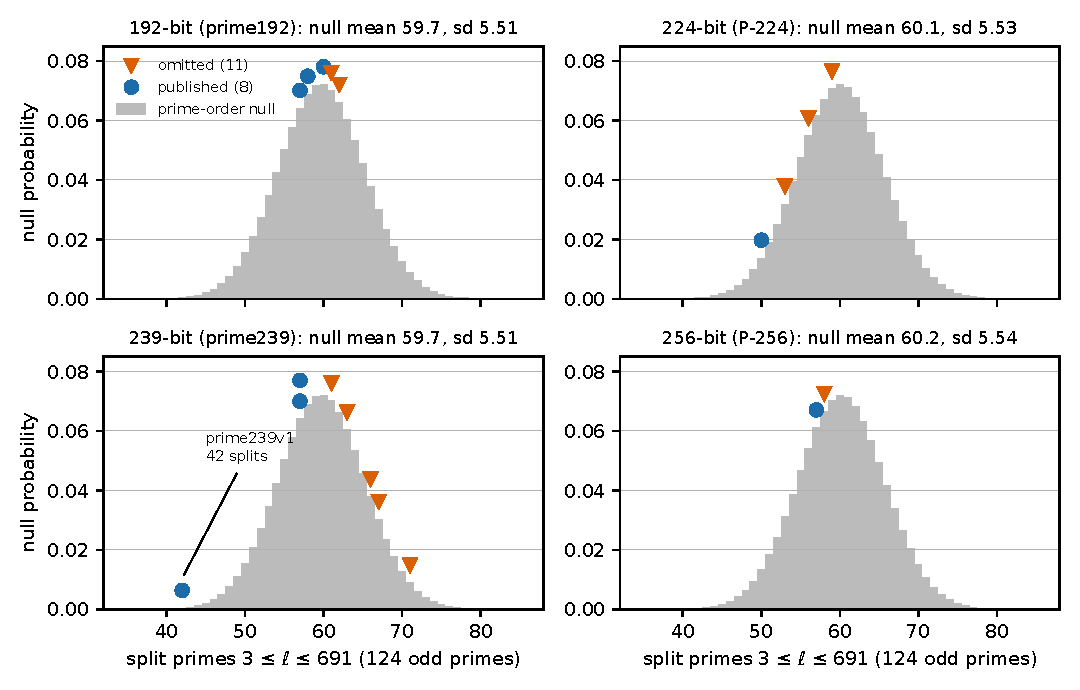
\includegraphics[width=\linewidth]{figures/fig_null.pdf}
\caption{Exact prime-order null for $S$ (grey) with the nineteen curves at
$B = 691$; omitted curves as triangles, published as circles. Source:
\texttt{S/runs/results.json}, \texttt{S/figures.py}.}
\label{fig:null}
\end{figure}

\begin{table}[ht]
\centering
\small
\begin{tabular}{lp{0.42\linewidth}p{0.36\linewidth}}
\toprule
Field & Omitted: $S$ (percentile) & Published: $S$ (percentile) \\
\midrule
192-bit & 61 (59.3), 62 (66.1) & v1 60 (52.2), v2 58 (38.0), v3 57 (31.3) \\
224-bit & 53 (10.1), 56 (23.1), 59 (42.3) & secp224r1 50 (3.4) \\
239-bit & 71 (97.9), 67 (90.6), 66 (87.2), 63 (72.3), 61 (59.2) & v1 \textbf{42 (0.06)}, v2 57 (31.2), v3 57 (31.2) \\
256-bit & 58 (34.8) & prime256v1 57 (28.4) \\
\bottomrule
\end{tabular}
\caption{Split counts and null mid-percentiles at $B = 691$
(Figure~\ref{fig:null}).}
\label{tab:pct}
\end{table}

\paragraph{Cutoff sweep} (Figure~\ref{fig:sweep}; data in
\path{S/runs/lookelsewhere.json} and \path{S/runs/permute.json}).
\begin{itemize}
\item The score reaches 25/25 only for $B \in \{691, 701, 709, 769\}$. At the
  other tabulated cutoffs (101, 251, 397, 997, 2003, 5003) it is 19--23,
  whether or not ramified primes or twist-forced splits are counted.
\item prime239v1 is most extreme near $B = 571$, at the 0.009th percentile. It
  stays below 1\% for $359 \le B \le 1367$ and reaches 11\% by $B = 5003$.
\end{itemize}

\begin{figure}[ht]
\centering
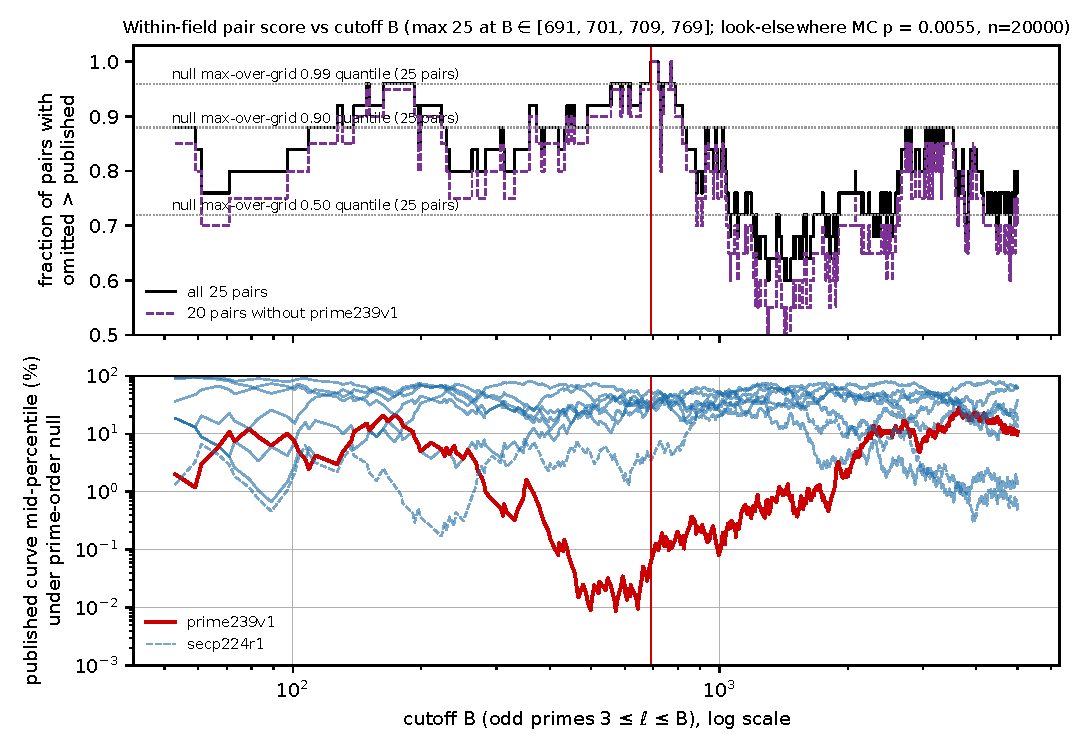
\includegraphics[width=\linewidth]{figures/fig_sweep.pdf}
\caption{Top: fraction of within-field pairs with the omitted curve above the
published one, against the cutoff $B$ (655 prime cutoffs); dotted lines are
null quantiles of the maximum over the grid. Bottom: the eight published
curves' null mid-percentiles. Source: \texttt{S/runs/lookelsewhere.json},
\texttt{S/runs/permute.json}.}
\label{fig:sweep}
\end{figure}

\paragraph{Correcting for the choice of $B$} (over 655 prime cutoffs).
\begin{itemize}
\item \emph{Random-curve null.} We drew 20{,}000 synthetic sets of nineteen
  prime-order curves (seed 20261029). The grid maximum of the pair score has
  null 0.50, 0.90 and 0.99 quantiles of 18, 22 and 24, and
  $P(\max \ge 25) = 0.0055$.
\item \emph{Exact label permutation} (4{,}480 allocations). $p = 0.0065$ for
  the grid maximum, and $1/4480$ at $B = 691$.
\item \emph{Without prime239v1.} The remaining 20 pairs score 20/20 on the
  same plateau, with a median of 15/20 over the grid.
\end{itemize}
These corrections do not cover the choice of statistic, which was formed after
many features had been examined on the same nineteen curves. They are
exploratory and had no protocol.

\section{Held-out test}\label{sec:heldout}

\paragraph{Protocol.} \path{S/PROTOCOL.md} was committed and pushed
(\texttt{bd5d146b}) before any held-out curve was computed. It fixes:
\begin{itemize}
\item the statistic: $S$ at $B = 691$ under the prime-order null;
\item the population;
\item one confirmatory test: within-field (held-out, published) pairs, the
  fraction with the held-out curve higher (ties count $\tfrac12$), and a
  one-sided within-field label-permutation $p$ from 200{,}000 draws;
\item the decision rule: the association replicates if $p \le 0.05$.
\end{itemize}
\path{S/AMENDMENT.md} corrects a count typo (48 for 42).
\path{S/protocol.json} transcribes the protocol into
\texttt{experiment.protocol/v1}. It validates but could not be frozen, because
the script was not hash-frozen before the data (deviation D3). The run also
launched without the required resume checkpoint (D1).

\paragraph{Primary result.} Held-out curves exceed published ones in
\textbf{0.574 of 102} pairs, with permutation $p = 0.29$. \textbf{The
association does not replicate} (Figure~\ref{fig:heldout}; rows in
\path{S/runs/rows.jsonl}).

\begin{figure}[ht]
\centering
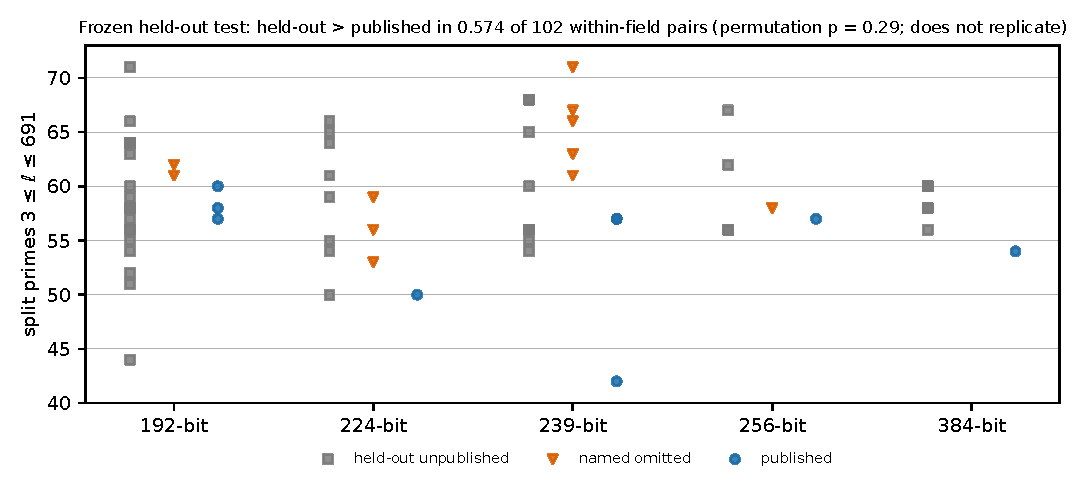
\includegraphics[width=\linewidth]{figures/fig_heldout.pdf}
\caption{Split counts at $B = 691$ by field: held-out unpublished curves
(squares), the named eleven (triangles) and published curves (circles), with
P-384 descriptive. Source: \texttt{S/runs/heldout.json}.}
\label{fig:heldout}
\end{figure}

\paragraph{Secondary results (descriptive).}
\begin{itemize}
\item The 42 held-out percentiles are consistent with uniform: KS $D = 0.153$
  against a 5\% critical value of 0.210.
\item The named eleven exceed the held-out curves in 0.630 of 115 pairs
  ($p = 0.13$).
\item Published P-384 (54 splits, 14.5th percentile) ranks lowest of the 7
  eligible curves in its field.
\item At the other six cutoffs the held-out-over-published fraction is
  0.66--0.71. This is reported, not tested.
\end{itemize}

\section{Discussion}\label{sec:discussion}

\paragraph{What the objections change.}
\begin{itemize}
\item \emph{Prime order.} The objection is right in principle but negligible
  here.
\item \emph{Forking paths.} This objection is borne out. Once the statistic is
  frozen and applied to curves it was not tuned on, the
  published-versus-unpublished difference is indistinguishable from chance.
\end{itemize}

\paragraph{What survives.} prime239v1 alone, with
$P(X \le 42) = 8.3 \times 10^{-4}$. The minimum over the 8 published curves
has null probability about 0.0066. Over all 61 eligible curves examined in the
four fields it is about 0.049, before any correction for $B$. An unpublished
192-bit curve reaches 44.

\paragraph{Mechanism.} None is known.
\begin{itemize}
\item No attack on prime-order curves, whether generic or rho, MOV/Frey--R\"uck,
  anomalous, Weil descent or index calculus, depends on how many rational small
  isogenies a curve has.
\item Within an isogeny class, ECDLP difficulty is uniform up to
  polynomial-time isogeny walks (Jao--Miller--Venkatesan~\cite{jmv}).
\item Elkies primes make SEA point counting \emph{faster}
  (Shparlinski--Sutherland~\cite{shparlinski-sutherland}). A designer avoiding
  slow counts would therefore favour \emph{more} splits, the opposite of the
  observed direction.
\end{itemize}

\paragraph{The CM field.} The only process story with any traction goes
through the CM field $K$. Write $\Delta = f_\pi^2 D_K$ with $D_K$ fundamental.
For $\ell \nmid f_\pi$, $(\Delta/\ell) = \chi_{D_K}(\ell)$, so $S$ counts the
primes $\ell \le 691$ that split in $K$. One might read a low $S$ as a small
$L(1, \chi_{D_K})$, and so a small class number, of the kind a CM-method
generator would produce. The $L$-value is in fact low, but not in a way that
supports the generator story.
\begin{itemize}
\item \emph{The direct test is $|D_K|$, and it fails.} A CM-method generator
  yields $|D_K|$ of a few million at most. The exact conductor census
  (\path{research/nist_seed_exact_conductor_census_20261023/}) factors
  $\Delta$ for all nineteen curves. It finds $f_\pi \in \{1, 3, 5\}$ and a
  smallest $|D_K|$ of about $2^{192.4}$ (an omitted 192-bit curve).
  prime239v1 has $f_\pi = 1$, so $D_K = \Delta$ and
  $|D_K| \approx 4p \approx 2^{241}$. An $L$-value cannot close this gap.
  Under GRH, $L(1,\chi)$ lies within a factor of about
  $(\log\log|D_K|)^{\pm 1}$ of~1~\cite{littlewood1928}. That is roughly 0.1 to
  18 here, so $h = \sqrt{|D_K|}\,L(1,\chi)/\pi$ stays within about $2^5$ of
  $\sqrt{|D_K|}/\pi$. A gap of about $2^{200}$ is out of reach. The
  class-group 2-ranks of the same nineteen fields overlap between published
  and omitted curves (\path{research/nist_seed_genus_rank_20261023/}).
\item \emph{$S$ is not an Euler product.}
  $\log L(1,\chi) \approx \sum_\ell \chi(\ell)/\ell$ is weighted by $1/\ell$,
  so the smallest primes dominate it. $S$ is an unweighted count, so the primes
  near the cutoff dominate it. Across the 61 eligible curves,
  $\operatorname{corr}(S(691), \log \Lhat) = 0.46$, while the weighted partial
  log-Euler product $E(691) = -\sum_{3 \le \ell \le 691} \log(1 - \chi(\ell)/\ell)$
  has $\operatorname{corr}(E(691), \log \Lhat) = 0.95$.
\item \emph{prime239v1's $L$-value is low (measured).} A follow-up study
  (\path{research/nist_seed_lvalue_20261030/}, protocol frozen before data)
  estimates $L(1, \chi_{D_K})$ by the Euler product to $x = 10^8$. Against
  exact class numbers of 20 random fundamental discriminants of 80--110 bits,
  this estimator is within $4 \times 10^{-5}$ in $\log L$. Under GRH the
  truncation error at $|D_K| \approx 2^{241}$ is expected to be about
  $10^{-3}$; this is not a proved bound. For prime239v1, $\Lhat = 0.246$, at
  the 0.25th percentile of the prime-order null and the lowest of the 61
  curves. Its partial log-Euler product is $-0.998$ over
  $3 \le \ell \le 691$ and only $+0.002$ over $\ell > 691$, so the first 124
  odd primes carry essentially all of it. $E(B)$ stays between the 0.22nd and
  0.25th percentile for $691 \le B \le 5003$. An independent study with
  separate code and a frozen protocol record
  (\path{research/nist_seed_l1chi_20261030/}) reproduces it: on the 61 shared
  curves $\log \Lhat$ at $x = 10^6$ agrees to $3 \times 10^{-14}$, and
  prime239v1 is again at the 0.25th percentile and the lowest
  (\path{CROSSCHECK.md} there). Over the same range, the split-count
  percentile rises from 0.06 to 11 (Section~\ref{sec:explore}). That rise is
  an artefact of the unweighted count, not a sign of an ordinary $L$-value.
\item \emph{It is the same anomaly, not new evidence.} prime239v1 was singled
  out because its $S$ was extreme, and $E(691)$ tracks $\log \Lhat$ closely.
  If nothing had been selected, some curve among 61 would reach the 0.25th
  percentile with probability $1 - (1 - 0.0025)^{61} \approx 0.14$ (about
  0.02 among the 8 published curves). The median $\log L$ percentiles are 39
  for the 8 published curves, 49 for the 11 omitted and 52 for the 42
  held-out curves. The 42 held-out percentiles fit the null (KS $D = 0.066$).
  The implied class number, $h \approx 2^{116.8}$, is within a factor of~2 of
  the null median. No known ECDLP method depends on $L(1,\chi)$ or on $h$.
\end{itemize}

\paragraph{Limitations.}
\begin{itemize}
\item The null assumes independence across $\ell$ and exact equidistribution.
\item The eight published curves are shared between the exploration and the
  test.
\item Monte Carlo $p$-values carry binomial error.
\item $\Lhat$ is a truncated Euler product, conditional on GRH for its
  expected accuracy; exact class numbers at $2^{241}$ were infeasible.
\end{itemize}

\bibliographystyle{plain}
\bibliography{refs}

\end{document}
